\documentclass[12pt,fleqn]{article}
\setlength{\parindent}{0pt}
\usepackage{graphicx}
\usepackage{cancel}
\usepackage{listings}
\usepackage[latin5]{inputenc}
\usepackage{color}
\setlength{\parskip}{8pt}
\setlength{\parsep}{0pt}
\setlength{\headsep}{0pt}
\setlength{\topskip}{0pt}
\setlength{\topmargin}{0pt}
\setlength{\topsep}{0pt}
\setlength{\partopsep}{0pt}
\setlength{\mathindent}{0cm}
\usepackage{showkeys}
\renewcommand*\showkeyslabelformat[1]{(#1)}

\begin{document}
Ders 18

Cift Entegrallerde Degisken Degisimi 

Ornek 

Bir elipsin alanini bulmak istedigimizi dusunelim. 

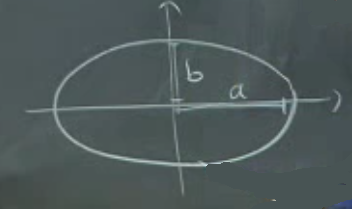
\includegraphics[height=2cm]{18_1.png}

\[ \bigg(\frac{x}{a}\bigg)^2 + \bigg(\frac{y}{b}\bigg)^2 = 1 \]

Formul cember formulune benziyor, tek fark $x,y$ kordinatlari farkli
sekillerde tekrar olceklenmisler (rescale). Elipsin alanini hesaplayalim. 

Diyelim ki 

\[ \int \int dx \ dy \]

olarak basladik. Ve

\[ \bigg(\frac{x}{a}\bigg)^2 + \bigg(\frac{y}{b}\bigg)^2 < 1 \]

olmak uzere $x,y$ uzerinden entegral alacagiz. Sinirlari ayarlamak,
vs. gibi islere hemen girisebiliriz, fakat bu is arap sacina donebilir. Bu
isi yapmanin en iyi yolu da degildir. 

Bu sekil bir cember olsaydi hemen kutupsal kordinata gecebilirdik, fakat
ustteki durumda bunu hemen yapamayiz. Fakat elips kenarlarindan bir basilmis
cemberdir, o zaman cemberi $a,b$ ile tekrar olceklersek, elips problemimizi
bir cember problemine indirgeyebiliriz. 

\[ \frac{x}{a} = u, \frac{y}{b} = v \]

O zaman alan soyle tanimlanabilir 

\[ \int \int_{u^2 + v^2 < 1} dx \ dy \]

Ama hala $dx,dy$ ile ne yapacagimiza karar vermedik. 

\[ du = \frac{1}{a}dx,dv = \frac{1}{b}dy \]

\[ du \ dv = \frac{1}{ab}dx \ dy \]

\[ dx \ dy = ab \ du \ dv \]

Entegrale sokarsak

\[ = ab \int \int_{u^2 + v^2 < 1} du \ dv \]

\[ = ab \cdot \textit{birim diskin alani} \]

\[ = \pi ab \]

Genel olarak yapmaya calistigimiz olcekleme faktorunun (scaling factor) ne
oldugunu bulmak, ki $dx \ dy$ ve $du \ dv$ arasindaki gecis mumkun olsun. 

Ornek 

\[ u = 3x - 2y \]

\[ v = x + y \]

Niye ustteki gibi $u,v$ kullanilmis? Belki entegre edilen fonksiyonu, belki
de sinirlari basitlestirmek istiyoruz. 

$dA = dx \ dy$, ya da $dA' = du \ dv$ 

Fakat bir problem var. Alan hesabinda entegralin ufak alan parcalarini
topladigini soylemistik. 

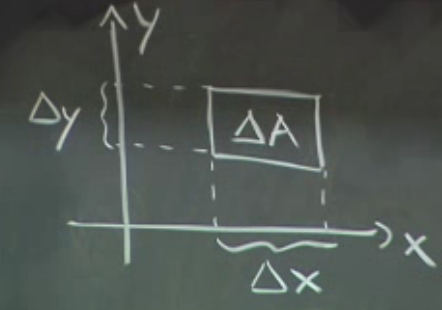
\includegraphics[height=2cm]{18_2.png}

Problem soyle, ustteki dikdortgen, bu ornegin donusum formullerine gore
$u,v$ baglaminda alttaki gibi bir sekle donusecek, yani paralelogram
olacak. 

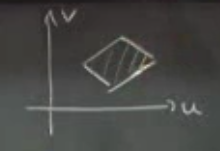
\includegraphics[height=2cm]{18_3.png}

Bir ornek uzerinde gorelim, her kenari 1 uzunlugunda kareyi alirsak

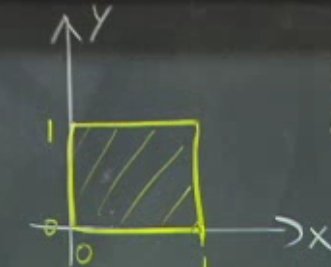
\includegraphics[height=3cm]{18_4.png}

ve bu karenin her noktasini $u,v$ formulleriyle donusturursek

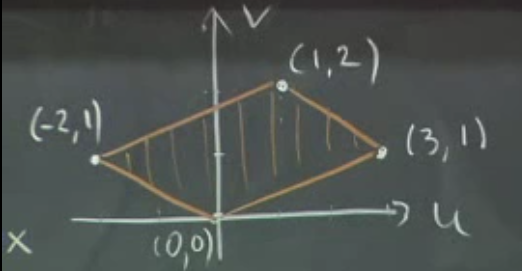
\includegraphics[height=3cm]{18_5.png}

elde edilir. Hakikaten bu bir paralelogram. 

















\end{document}
